\subsection{Architectural Patterns}

\subsubsection{Model-View-Presenter}
This project will primarily be using the Model-View-Presenter pattern for its architecture and will 
be using the JavaScript library Backbone to implement the pattern. Model-View-Presenter is a slightly
modified version of Model-View-Controller, made to work better with HTML and JavaScript. The Presenter
is a JavaScript object which connects a Backbone Model to the HTML object which serves as the View.

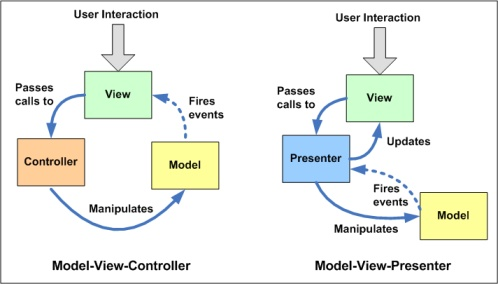
\includegraphics{pictures/mvc_mvp}

\subsubsection{Game Loop}
The game runs a loop using the JavaScript requestAnimationFrame function. This loop updates the parts 
of the game which needs to be updated and repaints the parts of the screen which needs to be repainted.

\subsubsection{Singletons}
There are 2 singleton objects in the game. One is an Image Library. This object is responsible for 
loading and storing the sprites the game will draw to the screen. This will allow us to only read and 
store each sprite one time, saving memory and improving performance. The second singleton object is 
the Object Pool. This object creates game objects, and stores them while they are not placed on the 
game map. This object will create all the objects when the game loads, so that they do not have to 
be created later, further improving performance. The Object Pool also prevents garbage collection 
from reducing the game's performance. Both these singletons are commonly used in video games.
